\section{Background}


In this section, we introduce the necessary background about the dynamic updates in the domain name system and its security considerations.

\subsection{Brief History}

The basic specification of the domain name system was introduced over 30 years ago \cite{rfc1035,rfc1034}. 
Before then, host name to address mappings were maintained by the Network Information Center (NIC) in a single file called \texttt{HOSTS.TXT} and distributed by all hosts using FTP \cite{rfc952,rfc953}.
%
The DNS protocol initially supported queries of a statically configured database that was updated manually as it was not expected to change rapidly \cite{rfc1034}. 
However, with the introduction of the Dynamic Host Configuration Protocol (DHCP) \cite{rfc2131}, which allows to dynamically assign an IP address to each device on a network, the automatic reconfiguration mechanism for DNS  became also essential.

\begin{figure}[!ht]
\centering
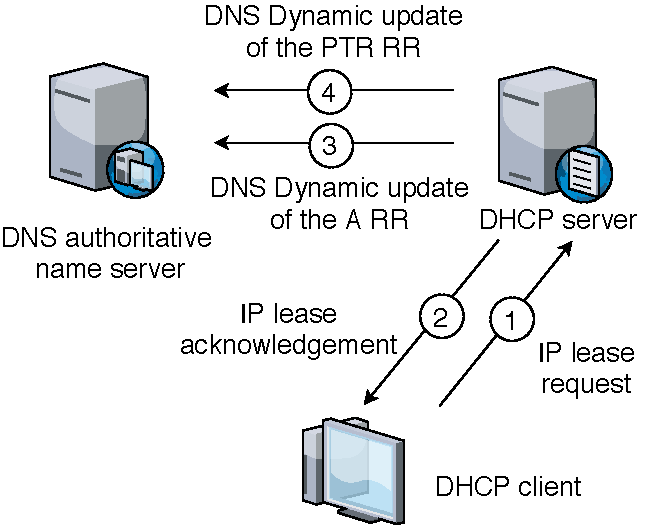
\includegraphics[width=2.5in]{figs/dhcp.pdf}
\caption{The DHCP server can be configured to register and dynamically update the host (\texttt{A}) and pointer (\texttt{PTR}) resource records with the authoritative DNS server of the zone on behalf of its DHCP-enabled clients.
%https://docs.microsoft.com/en-us/previous-versions/windows/it-pro/windows-server-2008-R2-and-2008/dd145315(v=ws.10)
}
\label{fig_dhcp}
\end{figure}

\subsection{Dynamic Updates in DNS}
%The DHCP protocol provides not only a mechanism for allocation of network addresses to Internet hosts but also can be configured to  dynamically update both the \texttt{A} and \texttt{PTR} (reverse DNS record) resource records in the DNS server on a client's behalf.

Internet services may use static IP addresses but can also dynamically change over short periods of time, on the order of hours or days \cite{gio}.
Due to the distributed nature of the domain mane system and the proliferation of its actors such as registrars or registry operators, updates to the global domain name system may take hours to propagate. 
%
\textit{Dynamic updates in DNS} is a protocol extension that addresses the problem of fast changes of DNS resource records in zone files, such as an \texttt{A} record, which provides a mapping between a domain name and an IP address.

The dynamic updates have been described in RFC 2136 \cite{rfc2136}. 
The specification supports all DNS record types.
Therefore, a client can update, add or delete any type of record, including \texttt{A}, \texttt{AAAA}, \texttt{NS}, or \texttt{TXT}.
It is often used %as an extension of
in combination with the DHCP protocol, which can be configured not only as a mechanism for allocation of network addresses to Internet hosts but also to dynamically update both \texttt{A} and \texttt{PTR} (pointer or reverse DNS) resource records in the DNS server %on a client's behalf 
on behalf of its clients (cf.~\autoref{fig_dhcp}).


%It supports all DNS record types, but often it is used only as an extension of the DHCP system, and in which the authorized DHCP servers register the client records in the DNS.


%
%Following this specification, a DNS client can add or delete any type of RR, such as A, AAAA, CNAME, or NS.

%Some servers that are maintained by certain types of Internet service providers (ISPs) are likely to change their IP address over very short periods of time, 



The proposed DNS \texttt{UPDATE} message complies with the standard DNS message format (cf. RFC 1035 \cite{rfc1035}) and is defined as follows:
\newline
\noindent
       \texttt{+----------------+}
      \newline \noindent
       \texttt{|\hspace{0.85cm} Header\hspace{0.85cm} |} contains the opcode value~(5)
      \noindent \texttt{+----------------+}
      \newline \noindent
      \texttt{|\hspace{1.16cm}Zone\hspace{1.16cm} |} specifies the zone to update
      \texttt{+----------------+}
      \newline \noindent
      \texttt{|~\hspace{0.115cm}~Prerequisite\hspace{0.115cm} |} RRs that must~(not)~preexist
      \texttt{+----------------+}
      \newline \noindent
      \texttt{|\hspace{0.95cm}Update\hspace{0.95cm} |} RRs to be added or deleted
      \texttt{+----------------+}
      \newline \noindent
      \texttt{|\hspace{0.005cm}Additional Data\hspace{-0.005cm} |} additional information (if any)
      \texttt{+----------------+}

The \texttt{Header} section contains the \texttt{UPDATE} opcode equal to~5. The \texttt{Zone} section must specify the zone name to update, i.e. a domain name (e.g.: \texttt{\url{example.com}}). The \texttt{Prerequisite} section can specify 
requirements %demanded as conditions for an update in terms of a DNS zone file content 
that must be satisfied by the DNS zone file such as existence or nonexistence of a specific resource record (RR). %, before being allowed to proceed with an update
The \texttt{Update} section contains resource record(s) to be added to or deleted from the DNS zone (e.g.:  \texttt{\url{example.com} A 10.10.10.10}), whereas \texttt{Additional Data} section can be used to supply a server with some additional information needed to, for example,  secure DNS update~\cite{rfc2136}.

When a primary master name server that supports dynamic updates receives an update request, it verifies whether all prerequisites (if any) defined by the requestor are met and whether restrictions (if any) regarding which hosts are permitted to make updates are met.
Note that if there are no restrictions defined by the DNS authoritative name server, anyone who knows the name of the zone (e.g.: \texttt{\url{example.com}}) and the name server (e.g.: \texttt{\url{ns1.example.com}}) for that zone is capable of updating its content by sending a single UDP datagram.
It can be tested using a standard \texttt{nsupdate} command\footnote{Dynamic DNS update utility: \url{https://linux.die.net/man/8/nsupdate}}.
%
%
The RFC specification also defines a case, where the request is sent to a DNS slave server that is authoritative for a given domain name.
The update request is expected to be forwarded towards the primary DNS server that can modify the zone file.

\subsection{Security Considerations}
The method described in RFC 2136 also includes a brief discussion of the security considerations and recommends using DNS Security Extensions (DNSSEC) digital signatures covering requests to secure dynamic updates and restrict requestors to those authorized to perform them %, for example, a local DHCP server 
(cf. RFC~2137~\cite{rfc2137} %, superseded by RFC~3007~\cite{rfc3007}).
and RFC~3007~\cite{rfc3007}).
If the public key security mechanism is not implemented, an authoritative name server is expected to accept the dynamic updates only from a statically preconfigured set of IP addresses.
The address match lists should be as restrictive as possible and limited to, for example, an IP address of a DHCP server.
An alternative security mechanism based on shared secret key (TSIG: Secret Key Transaction Authentication for DNS) and message authentication code was introduced three years later in RFC 2845 \cite{rfc2845} and became the most commonly used method in popular DNS software implementations.
%
%
The pressing need for DNS dynamic updates and the delayed introduction of the robust and lightweight security measures may explain a rapid uptake of the vulnerable by design, non-secure dynamic updates.
%why the vulnerable, non-secure implementations have

%and the protocol's simplicity caused a rapid uptake of the specification.


\subsection{Implementations of Dynamic Updates}

The common implementations of the DNS software, such as the open source Linux BIND \cite{bind} or the Microsoft Server DNS support vulnerable configurations, such as accepting requests from all hosts.
Some are vulnerable by default.
To date, all versions of  the Microsoft Server DNS support either an Active Directory--integrated zone, allowing only secure updates using extended TSIG or a standard primary DNS configuration that supports \textit{only} non-secure dynamic updates.
Interesting, Microsoft is aware of the vulnerability and informs the users willing to setup a non-secure implementation that ``Allowing nonsecure dynamic updates is a significant security vulnerability because updates can be accepted from untrusted sources.''
However, it remains unclear why the vulnerable version is still supported in the latest production version of the software--over 20 years after the initial release of the RFC specification.
